\documentclass{article}
\usepackage[utf8]{inputenc} % Allows UTF-8 encoding
\usepackage[T2A]{fontenc}   % Use T2A font encoding for Cyrillic
\usepackage[bulgarian]{babel} % Bulgarian language support
\usepackage{geometry}
\usepackage{graphicx}
\usepackage{titlesec}
\usepackage{fancyhdr}
\usepackage{threeparttable} % Добавете това в преамбюла
\usepackage{rotating} % Добавете това в преамбюла
\usepackage{tikz}
\usepackage{float} % Добавете това в преамбюла
\usepackage{graphicx} % Уверете се, че това е в преамбюла

\usetikzlibrary{shapes.geometric, arrows}

\geometry{a4paper, margin=1in}

% Персонализиран заглавен формат
\titleformat{\section}
  {\normalfont\Large\bfseries\centering}{\thesection}{1em}{}

% Заглавна част
\pagestyle{fancy}
\fancyhf{}
\fancyhead[L]{\textit{Epilepsia, 51(7):1177--1184, 2010}\\
doi: 10.1111/j.1528-1167.2009.02426.x}

\tikzstyle{startstop} = [rectangle, rounded corners, minimum width=3cm, minimum height=1cm, text centered, draw=black, fill=gray!30]
\tikzstyle{process} = [rectangle, minimum width=3cm, minimum height=1cm, text centered, draw=black, fill=gray!10]
\tikzstyle{arrow} = [thick,->,>=stealth]

\begin{document}

\setlength{\headheight}{23.10004pt}
% Заглавна кутия
\begin{center}
  \fbox{\parbox{\textwidth}{
    \centering
    \textbf{\large ПЪЛНО ДЪЛГО ОРИГИНАЛНО ИЗСЛЕДВАНЕ}
  }}
\end{center}

% Основно заглавие
\begin{center}
  \textbf{\LARGE Консумация на алкохол, непровокирани припадъци и епилепсия:}\\
  \textbf{\LARGE Систематичен преглед и мета-анализ}
\end{center}

% Автори
\begin{center}
  \textbf{*Андрий В. Самохвалов, *Хиацинт Ървинг, *Сатя Мохапатра и *†‡Юрген Рем}
\end{center}

% Афилиации
\begin{center}
  \textit{*Обществено здраве и регулаторна политика, Център за зависимост и психично здраве, Торонто, Онтарио, Канада;}\\
  \textit{†Училище за обществено здраве Дала Лана, Университет на Торонто, Торонто, Канада; и ‡Епидемиологично изследователско звено,}\\
  \textit{Клинична психология и психотерапия, Технически университет, Дрезден, Германия}
\end{center}

% Резюме
\section*{Резюме}
\textbf{Цел:} Целта на това изследване беше да анализира и количефицира връзката между консумацията на алкохол и епилепсията като самостоятелно заболяване, частично операционализирано чрез появата на непровокирани припадъци, както и да изследва причинността.\\
\textbf{Методи:} Систематичен преглед, мета-анализ.\\
\textbf{Резултати:} Открита е силна и последователна връзка между консумацията на алкохол и епилепсията/непровокираните припадъци с общ относителен риск (RR) от 2.19 [95\% доверителен интервал (CI) 1.83–2.63]. Имаше дозо-отговорна връзка между количеството консумиран алкохол дневно и вероятността за настъпване на епилепсия. Лица, консумиращи средно четири, шест и осем напитки дневно, имаха RR от 1.81 (95\% CI 1.59–2.07), 2.44 (95\% CI 2.00–2.97) и 3.27 (95\% CI 2.52–4.26), съответно, в сравнение с неконсумиращите. Бяха идентифицирани няколко патогенни механизма за развитието на епилепсия при потребителите на алкохол. Повечето от съответните изследвания установиха, че висок процент от потребителите на алкохол с епилепсия биха отговаряли на критериите за алкохолна зависимост. Данните бяха неубедителни относно прага за ефекта на алкохола, но повечето изследвания предполагат, че ефектът може да се прояви само при тежко пиене (четири и повече напитки дневно).\\
\textbf{Дискусия:} Връзката между консумацията на алкохол и епилепсията и непровокираните припадъци беше количефицирана и бяха предложени няколко патогенни механизма, въпреки че нито един от тях не е доказан като уникален причинен път за епилепсия. Определени ограничения, които стоят в основата на това изследване, изискват допълнителни изследвания, за да се изяснят оставащите статистически въпроси и патогенезата на епилепсията при тежки пиячи.\\
\textbf{КЛЮЧОВИ ДУМИ:} Алкохол, Тежко пиене, Алкохолна зависимост, Епилепсия, Непровокирани припадъци.

% Добавете този текст към документа
\section*{Въведение}
Епилепсията е едно от най-честите неврологични състояния, с годишна честота в индустриализираните страни от 40–70 на 100,000 души. Преобладаването на рецидивиращи непровокирани припадъци варира от 370 на 100,000 в Исландия до 800 на 100,000 в Полша и Фарьорските острови (Jallon, 2002). Жизнената честота на различните видове припадъци е много по-висока от честотата на активната епилепсия. Оценено е, че до 5\% от населението ще изпита нефебрилни припадъци в някакъв момент от живота си (Bell \& Sander, 2001). През 2000 г. епилепсията допринесе с повече от 7 милиона години на живот, коригирани с увреждания (DALYs), 0.5\% от глобалната тежест на заболяванията (Leonardi \& Ustun, 2002). Освен относително високата си честота, епилепсията е силно стигматизирано заболяване (Jacoby, 2002; Fernandes et al., 2004).

Консумацията на алкохол, един от петте най-важни рискови фактора за глобалната тежест на заболяванията и уврежданията (Ezzati et al., 2002; Rehm et al., 2003), е показано, че е свързана с епилепсия (English et al., 1995). Множество изследвания са изследвали сложната връзка между консумацията на алкохол и епилепсията, с основен фокус върху алкохол-индуцирани припадъци поради отнемане (Alldredge \& Lowenstein, 1993; Hillbom et al., 2003). Въпреки това, малко изследвания са изследвали настъпването на епилепсия като самостоятелно заболяване, както и появата на непровокирани припадъци сред потребителите на алкохол. И двата фактора могат да бъдат от решаващо значение за определяне на причинната роля на алкохола като самостоятелен рисков фактор за епилепсия. Това е в съответствие с възможността много събития, обозначени като епилепсия, да са алкохол-отнемащи припадъци, а не непровокирани припадъци. Това изследване имаше за цел да анализира и количефицира връзката и дозо-отговорната връзка между консумацията на алкохол и епилепсията, с особен фокус върху изследването на потенциални механизми.

\section*{Методи}
\textbf{Определение на резултата}

За това изследване използвахме определението за епилепсия, извлечено от Международната лига срещу епилепсия (ILAE) и Международното бюро за епилепсия (IBE). Според ILAE и IBE, епилепсията е разстройство на мозъка, което се характеризира с трайна предразположеност към генериране на епилептични припадъци. Това определение за епилепсия изисква появата на поне един епилептичен припадък (Fisher et al., 2005). В съответствие с това определение, включихме изследвания в мета-анализа, които съобщават за непровокирани припадъци или епилепсия като техни резултати.

\textbf{Систематично търсене на литературата и извличане на данни}

Компютърно базирано систематично търсене на литературата беше завършено, използвайки Ovid MEDLINE, EMBASE, Web of Science, CINAHL, PsychINFO, ETOH и Google Scholar. Периодът на търсене беше от януари 1960 до септември 2008 (извършено през октомври 2008), нямаше езикови ограничения и използваше всички комбинации от ключови думи: alcohol* (съкратено), alcohol, alcohol consumption, alcohol intake, drinking, alcoholism, alcohol abuse, alcohol misuse, epilep* (съкратено), epilepsy, epileptic, seizures. Освен това, основни епидемиологични списания и списъци с референции на съответни статии бяха прегледани ръчно.

Критериите за включване на прегледаните статии бяха:
\begin{enumerate}
  \item Дизайн на случай-контрол или кохортен дизайн.
  \item Включването на коефициенти на опасност (HRs), относителни рискове (RRs) или коефициенти на вероятност (ORs), с 95\% доверителни интервали (CIs) (или информация, позволяваща тяхното изчисление).
  \item Крайната точка е заболеваемостта от епилепсия (както е определено от лекар) или непровокирани припадъци.
  \item Три или повече категории на консумация на алкохол, докладвани (за анализ на дозо-отговор).
\end{enumerate}

Критериите за изключване бяха:
\begin{enumerate}
  \item Дизайн на напречно сечение или други дизайни без никакъв контрол.
  \item Данни, които не позволяват изчисление на риска за съответните променливи на експозиция.
  \item Изследвания, основно върху алкохол-индуцирани припадъци, както и всякакви припадъци, провокирани от други фактори (инсулти, възпаления и т.н.).
\end{enumerate}



Ако бяха намерени няколко публикувани доклада, базирани на едни и същи данни от изследването, в мета-анализа беше включено изследването с най-пълни данни за консумацията на алкохол. Търсенето на литературата доведе до 1,360 статии, 18 от които количествено определиха връзката между консумацията на алкохол и епилепсията. Ако изследването представяше информация отделно за различни кохорти от пациенти или категории на резултатите, данните бяха извлечени в отделни набори от данни. В изследванията на Leone et al. (1997) и Ng et al. (1988) информацията беше представена отделно за мъже и жени и беше извлечена като набори от данни (a) и (b) съответно за всяко изследване.

Изследването на Leone et al. (2002) предостави данни отделно за две различни кохорти от пациенти. Създадохме два набора от данни за това изследване: един за субекти с непровокирани симптоматични припадъци (набор от данни a) и друг за субекти с криптогенни/идиопатични припадъци (набор от данни b). Общо шест изследвания, включващи девет независими набора от данни, отговаряха на критериите за включване (виж Таблица 1). Подробна информация за избора на изследвания е представена на Фиг. 1. За статистически цели консумацията на алкохол беше преобразувана в средни грамове чист алкохол на ден. Средна стойност беше изчислена, когато консумацията на алкохол беше дадена в диапазони. В случаи на отворени категории, 75% от ширината на предишната категория диапазон беше добавена към долната граница на такива категории.

\textbf{Статистически мета-анализ}
Първо изследвахме връзката между консумацията на алкохол (всяко пиене срещу никакво пиене) и риска от епилепсия. За да направим това, обединихме относителните рискове (RRs) (претеглени според обратната стойност на тяхната дисперсия) за всички категории пиене от всяко изследване, за да извлечем единен RR за всяко изследване. Бяха изчислени естествените логаритми на RRs и беше използван модел с случайни ефекти, за да се извлече обобщен RR, сравняващ всяко пиене с никакво пиене (референтната категория) за всички комбинирани изследвания (DerSimonian \& Laird, 1986).
Също така завършихме друг категоричен мета-анализ, сравняващ RR на епилепсия за дневна консумация на алкохол под 50 г в сравнение с непиещите, за да идентифицираме потенциална прагова връзка (т.е. епилепсията е свързана само с тежко пиене). Обединихме RRs (претеглени според обратната стойност на тяхната дисперсия) за всички категории пиене под 50 г от всяко изследване, за да извлечем единен RR за всяко изследване, за да сравним с никакво пиене, използвайки същата методология, описана по-рано за дихотомията алкохол да/не. И двата категорични анализа бяха завършени, използвайки командата metan в STATA 10.1 (Stata Corporation, College Station, TX, U.S.A.).
За да оценим дозо-отговорната връзка между консумацията на алкохол и риска от епилепсия, използвахме метода, предложен от Грийнланд и др. (Greenland \& Longnecker, 1992; Orsini \& Greenland, 2006), за да изчислим обратно и обединим оценките на риска. Включени бяха само изследвания, които предоставиха броя на случаите и контролните групи, и RRs с оценки на дисперсията за три или повече количествени категории на експозиция на алкохол. За регресията използвахме средните стойности, описани по-рано. За да извлечем дозо-отговорната крива, използвахме семейство от първо- и второстепенни фракционни полиномиални модели (Royston \& Sauerbrei, 2008). Всички модели бяха съставени, използвайки модели с случайни ефекти (DerSimonian \& Laird, 1986). Най-добре пасващият модел беше избран въз основа на затворен тест за сравнение между фракционни полиномиални модели (Royston \& Sauerbrei, 2008), а общата пригодност на модела беше оценена с помощта на статистиката на Cochrane Q (Higgins \& Thompson, 2002; Higgins et al., 2003). Тези анализи бяха завършени, използвайки командата GLST в STATA 10.1

\small



% ... existing code ...
\begin{sidewaystable}[h]
  \centering
  \small % Reduce font size
  
  \caption{Характеристики на включените изследвания}
  \begin{threeparttable}
  \begin{tabular}{|p{2.5cm}|p{3cm}|p{1.5cm}|p{2cm}|p{1cm}|p{1cm}|p{7.5cm}|p{2cm}|}
  \hline
  \textbf{Автор(и)} & \textbf{Място и време на изследването} & \textbf{Пол} & \textbf{Дизайн на изследването} & \textbf{Случаи} & \textbf{Контроли} & \textbf{Категории на експозиция} & \textbf{Резултат} \\ \hline
  Zeng et al. (2003) & Китай, 2000 & И двата пола & Случай-контрол & 81 & 81 & Консумация на алкохол не е уточнена & Първична епилепсия \\ \hline
  Leone et al. (2002; a)\textsuperscript{a} & Италия, януари 1995--октомври 1998 & И двата пола & Случай-контрол & 33 & 59 & Настоящи въздържатели (пили не повече от веднъж годишно) и случайни пиячи (пили поне веднъж годишно, но по-малко от веднъж месечно); Настоящи пиячи, класифицирани по среден дневен прием на алкохол (>50 и $\leq$ 50 г/ден) & Непровокирани симптоматични припадъци \\ \hline
  Leone et al. (2002; b)\textsuperscript{a} & Италия, януари 1995--октомври 1998 & И двата пола & Случай-контрол & 139 & 220 & Настоящи въздържатели (пили не повече от веднъж годишно) и случайни пиячи (пили поне веднъж годишно, но по-малко от веднъж месечно); Настоящи пиячи, класифицирани по среден дневен прием на алкохол (>50 и $\leq$ 50 г/ден) & Идиопатични/Криптогенни припадъци \\ \hline
  Leone et al. (1997; a)\textsuperscript{a} & Италия, февруари 1992--октомври 1993 & Мъже & Случай-контрол & 152 & 296 & Настоящи въздържатели (пили не повече от веднъж годишно) и случайни пиячи (пили поне веднъж годишно, но по-малко от веднъж месечно); Настоящи пиячи, класифицирани по среден дневен прием на алкохол (1--25; 26--50; 51--100; 101--200; 200+ г/ден) & Генерализирани тонично-клонични припадъци \\ \hline
  Leone et al. (1997; b)\textsuperscript{a} & Италия, февруари 1992--октомври 1993 & Жени & Случай-контрол & 77 & 151 & Настоящи въздържатели (пили не повече от веднъж годишно) и случайни пиячи (пили поне веднъж годишно, но по-малко от веднъж месечно); Настоящи пиячи, класифицирани по среден дневен прием на алкохол (1--25; 26--50; 51--100; 101--200; 200+ г/ден) & Генерализирани тонично-клонични припадъци \\ \hline
  Leone et al. (1994) & Италия, януари 1990--март 1991 & И двата пола & Случай-контрол & 81 & 169 & Бивши пиячи (пили поне веднъж месечно и въздържали се поне 1 година); Пиячи, класифицирани по среден дневен прием на алкохол (>50 и $\leq$ 50 г/ден) & Непровокирани припадъци \\ \hline
  Ng et al. (1988; a)\textsuperscript{a} & САЩ, декември 1981--февруари 1984 & Мъже & Случай-контрол & 145 & 128 & Въздържатели (както настоящи, така и през целия живот); Пиячи, класифицирани по среден дневен прием на алкохол (1--50; 51--100; 101--200; 201--300; 300+ г/ден) & Непровокирани припадъци \\ \hline
  Ng et al. (1988; b)\textsuperscript{a} & САЩ, декември 1981--февруари 1984 & Жени & Случай-контрол & 71 & 139 & Въздържатели (както настоящи, така и през целия живот); Пиячи, класифицирани по среден дневен прием на алкохол (1--50; 51--100; 101--200; 201--300; 300+ г/ден) & Непровокирани припадъци \\ \hline
  Ogunniyi et al. (1987) & Нигерия, септември 1983--декември 1984 & И двата пола & Случай-контрол & 155 & 155 & Консумация на алкохол не е уточнена & Епилепсия \\ \hline
  \end{tabular}
  \begin{tablenotes}
  \item \textsuperscript{a}Няколко изследвания имаха два набора от данни, съответно наречени a и b. За статистически цели наборите от данни, взети от едно и също изследване, бяха използвани отделно.
  \end{tablenotes}
  \end{threeparttable}
\end{sidewaystable}

  \normalsize



  \begin{figure}[h]
      \centering
      \caption{Процес на подбор на изследвания. Epilepsia ILAE}
      \begin{tikzpicture}[node distance=2cm]
      
      \node (start) [startstop] {\parbox{3cm}{1360 резюмета идентифицирани \\ от основното търсене}};
      \node (exclude1) [process, below of=start, yshift=-0.5cm, xshift=-3cm] {\parbox{3cm}{1342 изследвания изключени \\ (няма релевантна информация)}};
      \node (relevant1) [startstop, right of=exclude1, xshift=5cm] {\parbox{3cm}{18 потенциално релевантни изследвания \\ идентифицирани и прегледани за извличане}};
      \node (exclude2) [process, below of=relevant1, yshift=-1cm, xshift=-4cm] {\parbox{3cm}{11 изследвания изключени \\ (замърсяване на базовата линия)}};
      \node (relevant2) [startstop, right of=exclude2, xshift=5cm, yshift=0.5cm] {\parbox{3cm}{7 потенциално релевантни изследвания \\ идентифицирани и прегледани за извличане}};
      \node (exclude3) [process, below of=relevant2, xshift=1cm, yshift=-0.5cm] {\parbox{3cm}{1 изследване изключено \\ (дублиране на резултати)}};
      \node (usable) [startstop, below of=exclude3, yshift=-1cm, xshift=-4cm] {\parbox{3cm}{6 изследвания бяха използваеми по отношение на \\ статистическо представяне и дефиниция на резултатите}};
      
      % Arrows
      \draw [arrow] (start) -- (exclude1);
      \draw [arrow] (start) -- (relevant1);
      \draw [arrow] (relevant1) -- (exclude2);
      \draw [arrow] (relevant1) -- (relevant2);
      \draw [arrow] (relevant2) -- (exclude3);
      \draw [arrow] (relevant2) -- (usable);
      
      \end{tikzpicture}
  \end{figure}
  

\section{Статистически анализ}

Статистическата хетерогенност между изследванията беше изследвана с помощта на статистиките на Cochrane Q и I\textsuperscript{2}. За статистиката Q, p-стойност <0.10 се счита за представителна за статистически значима хетерогенност. I\textsuperscript{2} представлява процента от общата вариация, допринесена от вариацията между изследванията. Тя варира между 0\% и 100\%, като стойности от 25\%, 50\% и 75\% се считат за представителни за ниска, умерена и висока хетерогенност, съответно (Higgins \& Thompson, 2002). Фуниеобразен график с псевдо 95\% CI беше използван за визуална оценка на публикационния пристрастие. За тестване на публикационния пристрастие използвахме командата STATA metabias, която изпълнява теста за асиметрия на регресията на Egger (Egger et al., 1997) и коригирания рангов корелационен тест на Begg (Begg \& Mazumdar, 1994). p-стойност <0.10 се счита за представителна за статистически значим публикационен пристрастие. Всички статистически анализи бяха извършени с помощта на STATA версия 10.1.

\section{Пътища}

В допълнение към формалния мета-анализ, който имаше за цел да количефицира дозо-отговорната връзка между консумацията на алкохол и риска от непровокирани припадъци и епилепсия, ние изследвахме патологичната етиология на такива връзки, по-специално биологични пътища, обратимост след интервенции, времеви и консистентност на асоциацията и релевантни експериментални изследвания.

\section{Резултати}

Мета-анализът на изследванията (Ogunniyi et al., 1987; Ng et al., 1988; Leone et al., 1994, 1997, 2002; Zeng et al., 2003) за риска от епилепсия при консумация на алкохол доведе до обединен RR от 2.19 (95\% CI 1.83–2.63) за всички изследвания (Фиг. 2). Нямаше значима хетерогенност между изследванията (Q-тест = 8.78, d.f. = 8 p = 0.361; I\textsuperscript{2} = 9\%, 95\% CI = 0–68\%). Визуалните инспекции на фуниеобразния график (Фиг. S1) и тестовете на Egger (p = 0.754) и Begg (p = 0.417) не показаха значима асиметрия. Тези резултати предполагат липса на съществен публикационен пристрастие.

Няколко изследвания (Ng et al., 1988; Leone et al., 1994, 1997, 2002) предоставиха данни, които ни позволиха да изследваме дозо-отговорната връзка между различните нива на редовна консумация на алкохол и началото на епилепсия. Най-добре пасващият модел може да се види на Фиг. 3. Статистиките за пасване на модела също показаха, че той предоставя добро пасване на данните (Q = 16.56, d.f. = 22, p = 0.787; I\textsuperscript{2} = 0\%, 95\% CI = 0–45\%). До точката от около 24 г алкохол на ден кривата между алкохола и риска от епилепсия беше относително плоска, след което обаче кривата на риска се увеличаваше рязко с увеличаващите се нива на консумация. Лицата, консумиращи 12, 48, 72 и 96 г алкохол дневно, имаха RR от 1.17 (95\% CI = 1.13–1.21), 1.81 (95\% CI = 1.59–2.07), 2.44 (95\% CI = 2.00–2.97) и 3.27 (95\% CI = 2.52–4.26), съответно, спрямо въздържателите.

Изследванията на Leone et al. (1994, 1997, 2002) установиха, че голям процент от хората с епилептични припадъци също са зависими от алкохол. Това ни доведе до въпроса дали само тежкото пиене е свързано с този проблем, тоест, има ли връзката между консумацията на алкохол и епилепсия праг? За да тестваме тази връзка, беше проведен категориен мета-анализ, включващ само изследвания, които имаха данни за <50 г дневна средна консумация на чист алкохол (около четири напитки). Този мета-анализ включваше четири изследвания, състоящи се от седем независими набора от данни (Ng et al., 1988; Leone et al., 1994, 1997, 2002).



\begin{figure}[H]
  \centering
  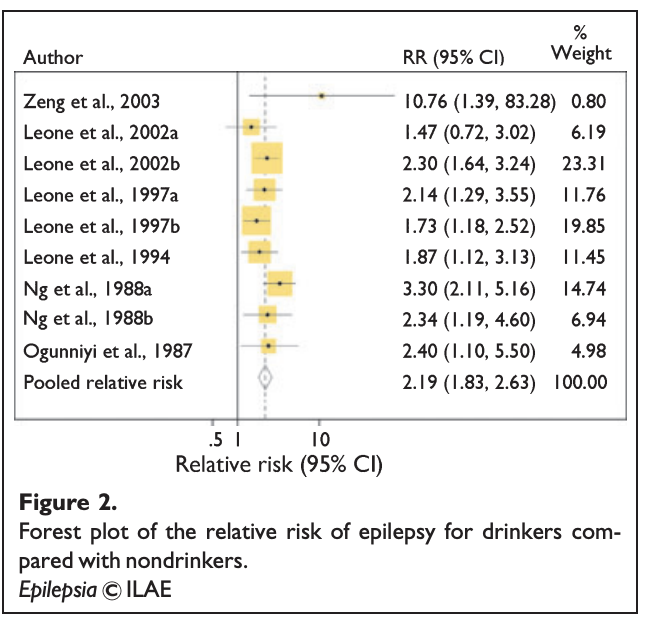
\includegraphics[width=\textwidth]{images/Screenshot 2024-10-22 at 10.11.42.png}
  \caption{Горски график на връзката между консумацията на алкохол и риска от епилепсия.}
  \label{fig:forest_plot}
\end{figure}

\begin{figure}[H]
  \centering
  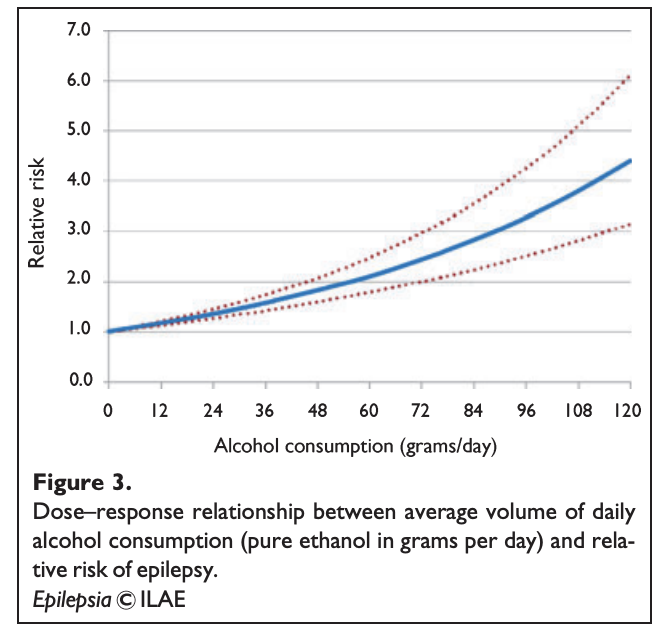
\includegraphics[width=\textwidth]{images/Screenshot 2024-10-22 at 10.12.52.png}
  \caption{Фуниеобразен график с псевдо 95\% CI за визуална оценка на публикационния пристрастие.}
  \label{fig:funnel_plot}
\end{figure}

\begin{figure}[H]
  \centering
  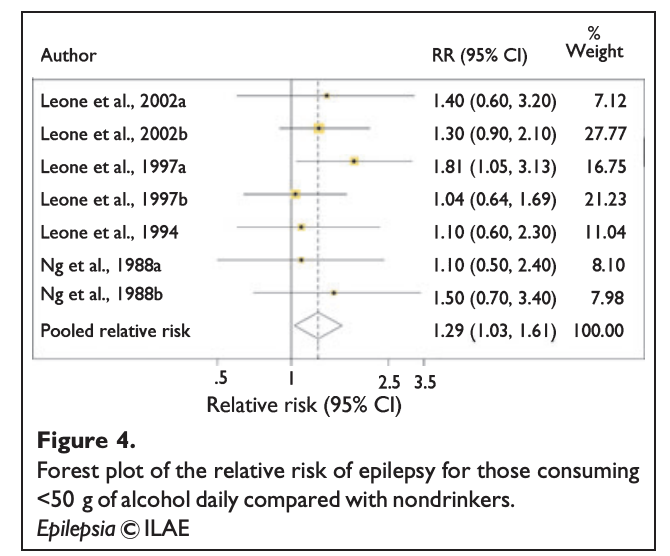
\includegraphics[width=\textwidth]{images/Screenshot 2024-10-22 at 10.13.21.png}
  \caption{Дозо-отговорна връзка между различните нива на редовна консумация на алкохол и риска от епилепсия.}
  \label{fig:dose_response}
\end{figure}


et al., 1988; Leone et al., 1994, 1997, 2002). Нямаше
доказателства за наличието на хетерогенност между
изследванията (Q = 2.79, d.f. = 6 p = 0.835; I\textsuperscript{2} = 0\%, 95\% CI =
0–71\%). Обобщеното RR за консумация под 50 г
алкохол дневно беше 1.29 (95\% CI = 1.03, 1.61) за всички
изследвания комбинирани (виж Фиг. 4).
Агрегирани над всички изследвания, резултатите показаха
леко повишен риск в сравнение с въздържателите, което
беше едва значимо (долна граница 1.03). 
Проблематичен
аспект на този резултат беше, че групата за сравнение включваше настоящи въздържатели. Следователно, може да е така,
че леко повишеният риск се дължи на ефекта на болните отказващи,
т.е. хора, които спират да пият по здравословни причини (Shaper et al., 1988).

\section{Дискусия}

\textbf{Ограничения на изследването}
Повечето от публикуваните изследвания включваха или бяха ограничени до припадъци при отнемане и само няколко изследвания бяха посветени изцяло на епилептични събития. Няколко изследвания, които включихме в мета-анализа, нямаха ясно определени резултати. Ng и сътр. (1988), например, съобщават за няколко вида припадъци, включително припадъци при отнемане. За да изключим последните, включихме подмножество от данни за непровокирани припадъци, които според авторите включват идиопатични и отдалечени симптоматични припадъци. Това беше същият подход, който използвахме за категориите непровокирани и идиопатични припадъци при извличане на данни от изследванията на Leone и сътр. (1994, 1997, 2002). Въпреки най-добрите ни усилия да извлечем съответните данни за неприпадъци при отнемане, някои данни за припадъци при отнемане на алкохол може все още да са включени в мета-анализа. Това може да е повлияло на дефиниционната яснота на мета-анализа. Следователно, по-нататъшни клинични изследвания са необходими, за да се направят причинно-следствените заключения по-ясни и окончателни.

\textbf{Хетерогенност на изследванията}
Изследванията, включени в мета-анализа, използваха различни резултати, които могат да бъдат разделени на две категории - епилепсия и първи припадъци. Признаваме, че комбинирането на такива резултати може да бъде спорно; въпреки това, използвахме данните за непровокирани припадъци с предположението, че ако припадъкът се случи без непосредствена причина, трябва да има мозъчна патология, която предразполага към повторение на припадъците. Според най-новата дефиниция на епилепсия от ILAE и IBE (Fisher и сътр., 2005), един припадък и наличието на предразполагащ фактор, т.е. появата на един припадък, може да се счита за начало на епилепсия в определени случаи. Въпреки че тази дефиниция все още е предмет на дискусия в научната литература, настоящите доказателства показват, че вероятността от повторение на припадъците при лица, които са имали един припадък, е висока (Fisher \& Lepik, 2008).

\textit{Асоциация и сила на асоциацията}
Мета-анализът на съществуващите случай-контрол изследвания
разкри ясна асоциация между консумацията на алкохол
и риска от поява на епилепсия или припадъци. Хетерогенността
на изследванията, отразяващи връзката между консумацията на алкохол и появата на припадъци или епилепсия в различни условия, е доказателство за последователността на тази асоциация.

\textit{Биологичен градиент и тестване на прага}
Съществуването на прагово отношение между консумацията на алкохол
и риска от епилепсия остава неустановено.
Въпреки това, намерихме доказателства за ясна дозо-отговорна връзка, както е отразено на Фиг. 3. Въз основа на статистическата част
на изследването можем ясно да заявим, че консумацията на алкохол е предразполагащ фактор за епилепсия и единични припадъци.
Въпреки това, са необходими допълнителни клинични изследвания преди по-


\textit{утвърдително заключение}
Може да се направи утвърдително заключение за причинно-следствената връзка между консумацията на алкохол и началото на епилепсия като самостоятелно заболяване.

\textit{Темпоралност}
Според клинични наблюдения, повтарящи се непровокирани припадъци се появяват след 10 или повече години на тежка консумация на алкохол (Devetag et al., 1983). Моделът на епилепсия, свързан с хронична консумация на алкохол, предложен от Bartolomei, съответства на този времеви период (Bartolomei, 2006). Въпреки това, тази теория се основава основно на хипотезата за „kindling“, която не може да се счита за уникален биологичен път за развитие на епилепсия при хронични алкохолици.

\textit{Правдоподобност и съгласуваност}
Хроничната консумация на алкохол има разнообразни ефекти върху централната нервна система, засягайки нейната структура и функциониране по няколко начина. Съществуват теории, обясняващи епилептогенезата при алкохолиците, включително мозъчни травми, хипоксия и kindling; всяка от тях е накратко описана по-долу. Dam и колеги наблюдават, че 74% от дългогодишните тежки алкохолици с епилепсия имат мозъчна атрофия като следствие от хроничната консумация на алкохол. Позиционирането на мозъчната атрофия като предразполагащ фактор за началото на епилепсия им позволи да я свържат като причинно-следствена връзка между консумацията на алкохол и епилепсията (Dam et al., 1985). Въпреки това, сравнително изследване на алкохолни пациенти (с поне 3-годишна история на алкохолизъм, средно 8 години) с и без епилепсия разкрива сходни нива на мозъчна атрофия и в двете групи, макар че мозъчната атрофия при алкохолиците с епилепсия е по-генерализирана. Това доведе авторите до заключението, че по-генерализираните форми на мозъчна атрофия могат да причинят епилепсия при алкохолиците (Meyer-Wahl & Braun, 1982). Други структурни промени като мозъчносъдови инфаркти, лезии и травми на главата са по-чести при тежки алкохолици и хора с алкохолна зависимост и са докладвани като пряка причина за повтарящи се епилептични припадъци в множество изследвания (Dam et al., 1985; Rathlev et al., 2006).

Теорията за „kindling“, предложена от Ballenger и Post, гласи, че повтарящото се отнемане, включително естественото отнемане чрез сън през годините, води до постепенно понижаване на епилептогенния праг (Ballenger \& Post, 1978). Въпреки че тази теория е най-правдоподобното обяснение за ефектите на етанола върху централната нервна система (ЦНС), тя не включва други фактори, описани по-рано, които на свой ред не могат да бъдат напълно изключени от анализа.

Появата на припадъци при алкохолиците може също да се обясни с определени промени в невротрансмитерните системи и метаболизма (йонен дисбаланс и хипогликемия), които причиняват хипервъзбудимост. Една от най-важните от тези промени е подрегулацията на експресията на гама-аминомаслена киселина (GABA)A рецептори, при която намаляването на чувствителността на GABA рецепторите съответства на намаляване на инхибиторното действие, свързано с GABA (Frye \& Fincher, 1988).

\textit{Обратимост след лечение}
Систематично търсене на клинични изпитвания, демонстриращи
подобрения на симптомите на епилепсия при потребители на алкохол
чрез лечение не доведе до никакви проучвания, подкрепящи
обратимостта на епилепсията.

\textit{Експериментални доказателства}
Поради етични причини, експерименталните доказателства за предизвикани от алкохол припадъци и епилепсия са ограничени до проучвания върху животни.
По-специално, многократните отнемания бяха свързани с
началото на спонтанни припадъци и корелираха с продължителността и количеството на отнеманията и понижаването на конвулсивния праг при плъхове (Kokka et al., 1993). Освен това,
Скорца и съавтори показаха, че отнемането на алкохол е
решаващо събитие за развитието на функционални и невропатологични изменения, свързани с епилепсия (Scorza
et al., 2003). Въпреки че проучванията върху животни са информативни по отношение на алкохол-свързаната епилептогенеза, откритията не могат
лесно да бъдат екстраполирани върху хора.

В обобщение, настоящите доказателства показват силна и последователна връзка между консумацията на алкохол и епилепсия или непровокирани припадъци, въпреки че тази връзка и нейната сила могат да бъдат уточнени в бъдещи изследвания, които също могат да включват идентифицирането на праг. Съществуващите изследвания ни позволиха да изчислим дозо-отговорната връзка за количеството редовно консумиран алкохол и риска от развитие на епилепсия или непровокирани припадъци при хронични алкохолици. Бяха предложени няколко патогенни механизма за развитието на епилепсия при тежки пиячи.

\section{Заключения}
Дозо-отговорната връзка между консумацията на алкохол и епилепсия и непровокирани припадъци беше количествено определена и бяха предложени няколко патогенни механизма, въпреки че нито един от тях не е показан като уникален причинен път за епилепсия. Определени ограничения на това изследване изискват допълнителни изследвания, за да се изяснят оставащите статистически въпроси и патогенезата на епилепсията при тежки пиячи.

\section{Благодарности}
Тази работа беше финансово подкрепена от договор \# HHSN267200700041C от NIAAA „Алкохол- и наркотично-атрибутивна тежест на болестите и нараняванията в САЩ“ и малък принос на изследването за глобалната тежест на болестите (GBD) към последния автор. Бихме искали да благодарим на Робин Рум, Тео Вос и основната група на сравнителната оценка на риска в рамките на изследването GBD 2005 за алкохол за подкрепата и коментарите относно общата методология и по-ранна версия на тази статия. Освен това, бихме искали да благодарим на Фотис Кантерес за редактирането на тази статия. Потвърждаваме, че сме прочели позицията на списанието по въпросите, свързани с етичното публикуване, и потвърждаваме, че този доклад е в съответствие с тези насоки.

\section{Разкритие}
Нито един от авторите няма конфликт на интереси за разкриване.


\section{Референции}
Alldredge BK, Lowenstein DH. (1993) Статус епилептикус, свързан със злоупотреба с алкохол. Epilepsia 34:1033–1037.

Ballenger JC, Post RM. (1978) Kindling като модел за синдроми на отнемане на алкохол. Br J Psychiatry 133:1–14.

Barclay GA, Barbour J, Stewart S, Day CP, Gilvarry E. (2008) Неблагоприятни физически ефекти от злоупотребата с алкохол. Advances in Psychiatric Treatment 14:139–151.

Bartolomei F. (2006) Епилепсия и алкохол. Epileptic Disord 8:S72–S78.

Begg CB, Mazumdar M. (1994) Оперативни характеристики на тест за рангов корелация за пристрастие при публикации. Biometrics 50:1088–1101.

Bell GS, Sander JW. (2001) Епидемиология на епилепсията: размерът на проблема. Seizure 10:306–314.

Brennan FN, Lyttle JA. (1987) Алкохол и припадъци: преглед. J R Soc Med 80:571–573.

Dam AM, Fuglsang-Frederiksen A, Svarre-Olsen U, Dam M. (1985) Епилепсия с късно начало: етиологии, видове припадъци и стойност на клиничното изследване, ЕЕГ и компютърна томография. Epilepsia 26:227–231.

DerSimonian R, Laird N. (1986) Мета-анализ в клинични изпитвания. Control Clin Trials 7:177–188.

Devetag F, Mandich G, Zaiotti G, Toffolo GG. (1983) Алкохолна епилепсия: преглед на серии и предложена класификация и етиопатогенеза. Ital J Neurol Sci 4:275–284.

Egger M, Smith GD, Schneider M, Minder C. (1997) Пристрастие в мета-анализ, открито чрез прост, графичен тест. BMJ 315:629–634.

English D, Holman C, Milne E, Winter M, Hulse G, Codde G, Bower G, Corti B, de Klerk N, Knuiman M, Kurinczuk J, Lewin G, Ryan G. (1995) Количествено определяне на заболеваемостта и смъртността, причинени от наркотици в Австралия 1995. Commonwealth Department of Human Services and Health, Canberra, Australia.

Ezzati M, Lopez AD, Rodgers AD, Vander Horn S, Murray CJL, Comparative Risk Assessment Collaborating Group. (2002) Избрани основни рискови фактори и глобална и регионална тежест на болестите. Lancet 360:1347–1360.

Fernandes PT, Salgado PCB, Noronha ALA, Barbosa FD, Souza EAP, Li LM. (2004) Скала за стигма на епилепсия: концептуални въпроси. J Epilepsy Clin Neurophysiol 10:213–218.

Fisher RS, van Emde Boas W, Blume W, Elger C, Genton P, Lee P, Engel J. (2005) Епилептични припадъци и епилепсия: дефиниции, предложени от международната лига срещу епилепсия (ILAE) и международното бюро за епилепсия (IBE). Epilepsia 46:470–472.

Fisher RS, Lepik I. (2008) Дебат: Кога припадъкът означава епилепсия? Epilepsia 49:7–12.

Frye GD, Fincher AS. (1988) Ефект на етанола върху натрупването на GABA, индуцирано от гама-винил GABA в substantia nigra и върху съдържанието на GABA в синаптозомите в шест мозъчни области на плъхове. Brain Res 449:71–79.

Greenland S, Longnecker MP. (1992) Методи за оценка на тенденциите от обобщени данни за дозо-отговор, с приложения към мета-анализ. Am J Epidemiol 135:1301–1309.

Higgins JP, Thompson SG. (2002) Количествено определяне на хетерогенността в мета-анализ. Stat Med 21:1539–1558.

Higgins JP, Thompson SG, Deeks JJ, Altman DG. (2003) Измерване на несъответствието в мета-анализи. BMJ 327:557–560.

Hillbom M, Pieninkeroinen I, Leone M. (2003) Припадъци при пациенти, зависими от алкохол. CNS Drugs 17:1013–1030.

Jacoby A. (2002) Стигма, епилепсия и качество на живот. Epilepsy Behav 3:10–20.

Jallon P. (2002) Епилепсия и епилептични разстройства, епидемиологичен маркер? Приноси на описателната епидемиология. Epileptic Disord 4:1–13.

Kokka N, Sapp DW, Taylor AM, Olsen RW. (1993) Моделът на kindling за алкохолна зависимост: подобно устойчиво намаляване на прага на припадъци към пентиленететразол при животни, получаващи хроничен етанол или хроничен пентиленететразол. Alcohol Clin Exp Res 17:525–531.

Leonardi M, Ustun TB. (2002) Глобалната тежест на епилепсията. Epilepsia 43:21–25.

Leone M, Bottacchi E, Gionco M, Nardozza V, Sironi L. (1994) Алкохол и епилептични припадъци: проучване на случай-контрол. Alcologia 6:215–219.

Leone M, Bottachi E, Beghi E, Morgando E, Mutani R, Amedeo G, Cremo R, Gianelli M, Ravagli Ceroni L. (1997) Употребата на алкохол е рисков фактор за първи генерализиран тонично-клоничен припадък. Neurology 48:614–620.

Leone M, Bottacchi E, Beghi E, Morgando E, Mutani R, Cremo R, Ravagli Ceroni L, Floriani I. (2002) Рискови фактори за първи генерализиран тонично-клоничен припадък в зряла възраст. Neurol Sci 23:99–106.

Meyer-Wahl JG, Braun J. (1982) Епилептични припадъци и мозъчна атрофия при алкохолици. J Neurol 228:17–32.

Ng SKC, Hauser AW, Brust JCM, Susser M. (1988) Консумация на алкохол и отнемане при новопоявили се припадъци. N Engl J Med 319:666–673.

Ogunniyi A, Osuntokun BO, Bademosi O, Adeuja AOG, Schoenberg BS. (1987) Рискови фактори за епилепсия: проучване на случай-контрол в Нигерия. Epilepsia 28:280–285.

Orsini NBR, Greenland S. (2006) Обобщени най-малки квадрати за оценка на тенденциите на обобщени данни за дозо-отговор. Stata J 6:40–57.

Rathlev NK, Ulrich AS, Delanty N, D’Onofrio G. (2006) Припадъци, свързани с алкохол. J Emerg Med 31:157–163.

Rehm J, Room R, Monteiro M, Gmel G, Graham K, Rehn N, Sempos C, Jernigan D. (2003) Алкохолът като рисков фактор за глобалната тежест на болестите. Eur Addict Res 9:157–164.

Royston P, Sauerbrei W. (2008) Многофакторно моделиране: прагматичен подход към регресионния анализ, базиран на фракционни полиноми за моделиране на непрекъснати променливи. John Wiley \& Sons, Hoboken, NJ.

Scorza FA, Arida RM, Cysneiros RM, Priel MR, de Albuquerque M, Cavalheiro EA. (2003) Ефектите на приема и отнемането на алкохол върху честотата на припадъците и хипокампалната морфология при плъхове с епилепсия. Neurosci Res 47:323–328.

Shaper A, Wannamethee G, Walker M. (1988) Алкохол и смъртност при британски мъже: обяснение на U-образната крива. Lancet 2:1267–1273.

Tsai G, Coyle JT. (1998) Ролята на глутаматергичната невротрансмисия в патофизиологията на алкохолизма. Annu Rev Med 49:173–184.

Zeng J, Zhen H, Mao-Sheng H, Mei-Hua J. (2003) Проучване на случай-контрол за рисковите фактори и други социо-психологически фактори на епилепсията. Chin J Epidemiol 24:116–118.

\section*{Поддържаща информация}
Допълнителна поддържаща информация може да бъде намерена в
онлайн версията на тази статия:
\begin{itemize}
  \item Фигура S1. Фуниеобразен график на Begg. Ln RR, естествен логаритъм
  на относителния риск; SE, стандартна грешка.
\end{itemize}
Моля, обърнете внимание: Wiley-Blackwell не носи отговорност за
съдържанието или функционалността на всяка поддържаща информация, предоставена от авторите. Всички запитвания (с изключение на липсващ материал) трябва да бъдат насочени към съответния автор на
статията.


\end{document}